\chapter{Understanding the capabilities of the OpenFlow protocol}
\ifpdf
    \graphicspath{{Chapter1/Chapter1Figs/PNG/}{Chapter1/Chapter1Figs/PDF/}{Chapter1/Chapter1Figs/}}
\else
    \graphicspath{{Chapter1/Chapter1Figs/EPS/}{Chapter1/Chapter1Figs/}}
\fi

This chapter contains the results of an exhaustive study over the capabilities
of existing SDN technologies and architectures. The work focuses on the
functionality of version 1.0 of the \of protocol as this is the sole
standardised instantiation of the SDN paradigm and version 1.0 is the current
standard that is provided by hardware switch firmware. In this work, \of
functionality is modular, thus the work can over 
other future protocol specification.  For this work, we have developed two frameworks:
\oflops and \sdnsim. \oflops is a high precision \of switch micro-benchmark
platform. Using the platform, we develop a set of elementary testing scenario in
order to understand the performance limitation of existing \of switch implementations.
\sdnsim is a macro-benchmark platform for \of architectures. The platform
extends the Unikernel abstraction in order to support large scale network
simulation and emulation, with the same code base. In this chapter I present in
Section~\ref{sec:oflops-intro} an introduction on the \oflops platform, 

% SDN context
% Driven by the OpenFlow
% initiative\footnote{\url{http://www.openflow.org/}}, the
% Software-Defined Networking (SDN) paradigm is gearing towards the
% definition of a standard way of providing pragrammatic control of
% network devices. Recently, the Open Networking Foundation
% \footnote{\url{http://www.opennetworkingfoundation.org/}} (ONF) was
% formed and is supported by major Internet companies including
% Microsoft, Google, Facebook, Cisco, Juniper, and VMware. With the
% ONF's first priority being to develop and use the OpenFlow protocol, a
% large number of commercial hardware platforms can be expected to
% become SDN-enabled in the near future.

% intro about SDN
\section{\oflops introduction} \label{sec:oflops-intro}

% OpenFlow\footnote{\url{http://www.openflow.org/}}, an instance of
% software-defined networking (SDN), gives access deep within the network
% forwarding plane while providing a common, simple, API for network-device
% control. Implementation details are left to the discretion of each vendor. This
% leads to an expectation of diverse strengths and weaknesses across the existing
% OpenFlow implementations, which motivates our work.


As we have discussed in Chapter~\ref{ch:background}, SDN techology can
enhance the functional capabilities of a network and provide high resolution 
flow control mechanisms in order to fulfil network application requirements. 
Although the short period since the introduction of the SDN paradigm, 
many novel control architectures have been proposed~\cite{plug_n_serv,difane,flowvisor-osdi}. 
One the most successful instantiations of the SDN paradigm is the \of protocol, 
standardized and developed by a joint consortium of educational and industrial
institutes, the Open Network Foundation (ONF). Currently \of is the sole SDN 
protocol that provides production support from a wide range of network vendors, 
while educational funding in US~\cite{ofelia} and Europe~\cite{ofelia} have 
develops large scale \of testbeds in order to support earch nnovativation in the
field.
%\of is increasingly adopted, both by hardware vendors as well as by the
%research community \cite{plug_n_serv,difane,flowvisor-osdi}.

In order though to make the transition of SDN and \of from research to industry
,  developers need to evaluate thoroughly proposed functionality and provide
accurate availability and performance guarantees.  Nonetheless, since the SDN
paradigm distributes control plane logic across various independent functional
units, performance evaluation is a difficult tasks. In order to address this
issue we developed \oflops~\footnote{\oflops is under GPL licence and can be
  downloaded from \url{http://www.openflow.org/wk/index.php/Oflops}}, a
measurement framework that enables rapid development of use-case tests for both
hardware and software OpenFlow switch implementations. To better understand the
behavior of the tested OpenFlow implementations, \oflops combines measurements
from the OpenFlow control channel with data-plane measurements. To ensure
sub-millisecond-level accuracy of the measurements, we bundle the \oflops
software with specialized hardware in the form of the NetFPGA
platform\footnote{\url{http://www.netfpga.org}}.  Note that if the tests do not
require millisecond-level accuracy, commodity hardware can be used instead of
the NetFPGA \cite{pam-accuracy}.

% We use \oflops to test publicly available OpenFlow software
% implementations as well as several OpenFlow-enabled commercial hardware
% platforms, and report our findings about their varying performance
% characteristics.  

% I would remove the following paragraph, this is not very relevant.
%The SDN concept has been employed by several authors to introduce innovation 
% in the forwarding behavior of the network. For example, 
%Greenhalgh~\etal.~\cite{flowstream} build a flexible flow
%processing platform based on commodity hardware. Handigol~\etal~\cite{plug_n_serv} 
%demonstrate a Web traffic load-balancer based on OpenFlow. 
%Yu~\etal~\cite{difane} scale
%flow-switching in an enterprise network by distributing the flow rules
%across the different switches. Sherwood~\etal~\cite{flowvisor-osdi}
%augment OpenFlow with flow-space isolation.


% What we propose in this paper: exploit the SDN paradigm to measure SDN capabilities.
%\todo{reviewer: you either make the case that SDN has "more and more promising use-cases" 
%or you say that you want to "help SDN become relevant"}
%While more and more promising use-cases for SDN technology are being
%proposed, the capabilities and performance delivered by SDN-enabled
%hardware is largely unknown. The history of networking has repeatedly
%reminded the research community that it takes time between innovations
%are proposed and the corresponding real-world applications are being
%deployed, e.g., multicast, VoIP, IPv6. To help SDN become a relevant
%technology in the real-world, we propose a framework that allows
%SDN-based application developers to test the actual capabilities of
%SDN hardware.

% The rest of this paper is structured as follows. We first present the design
% of the \oflops framework in Section~\ref{sec:design}. We describe the 
% measurement setup in Section~\ref{sec:switches}. We describe our measurements
% in Section~\ref{sec:results}. We provide basic experiments that test the flow
% processing capabilities of the implementations (Section~\ref{sec:results-packets})
% as well as the performance and overhead of the OpenFlow communication channel 
% (Section~\ref{sec:results-rate}). We follow with specific tests, targeting the monitoring
% capabilities of OpenFlow (Section~\ref{sec:results-monitoring}) as well as interactions
% between different types of OpenFlow commands (Section~\ref{sec:results-interactions}).
% We conclude in Section~\ref{sec:conclusion}.
% Rest of this paper...

\section{\oflops design}\label{sec:oflops-design}

Measuring OpenFlow switch implementations is a challenging task in terms of
characterization accuracy, noise suppression and precision.  Performance
characterization is not trivial as most OpenFlow-enabled devices provide rich
functionality but do not disclose implementation details. In order to understand
the performance impact of an experiment, multiple input measurements must be
monitored concurrently. Further, current controller designs,
like~\cite{Gude08,SNAC}, target production networks and thus are optimized for
throughput maximization and programmability, but incur high measurement
inaccuracy. Measurement noise suppresion in the control plane requires 
a new simplified \of controller library with low processing
latency. Finally, high precision measurements after a point are subject to loss
due to unobserved parameters of the measurement host, such as OS scheduling and
clock drift. The result of these challenges is that meaningful, 
controlled, repeatable performance tests are non-trivial in an \of
environment.

% Since the beggining of our measurement study, it became apparent to us
% that the assesment of OpenFlow implementations is not trivial and it
% has a number of challenges.  Firstly, in order to assess the
% performance and understand the limitations of a network device that
% has both rich functionality and for which we have little idea of the
% implementation, multiple input measurement should be monitored
% concurently in order to encompass all parameters of an
% experiment. Secondly, OpenFlow controllers like \cite{Gude08,SNAC}
% provide advanced APIs that support fine-grained control of the switch,
% through extensions based upon language mechanisms such as C++ bindings
% to Python. As a result, such extensions introduce processing
% complexity on the control channel which may introduce measurement
% noise, making them inappropriate for our measurements. Finally, for
% some of our measurements we required fine time precision, which after
% a point is subject to losses due to measurement host parameters, such
% as OS scheduling.


\begin{figure}
\centering
\begin{minipage}[b]{0.49\linewidth}
\centering
 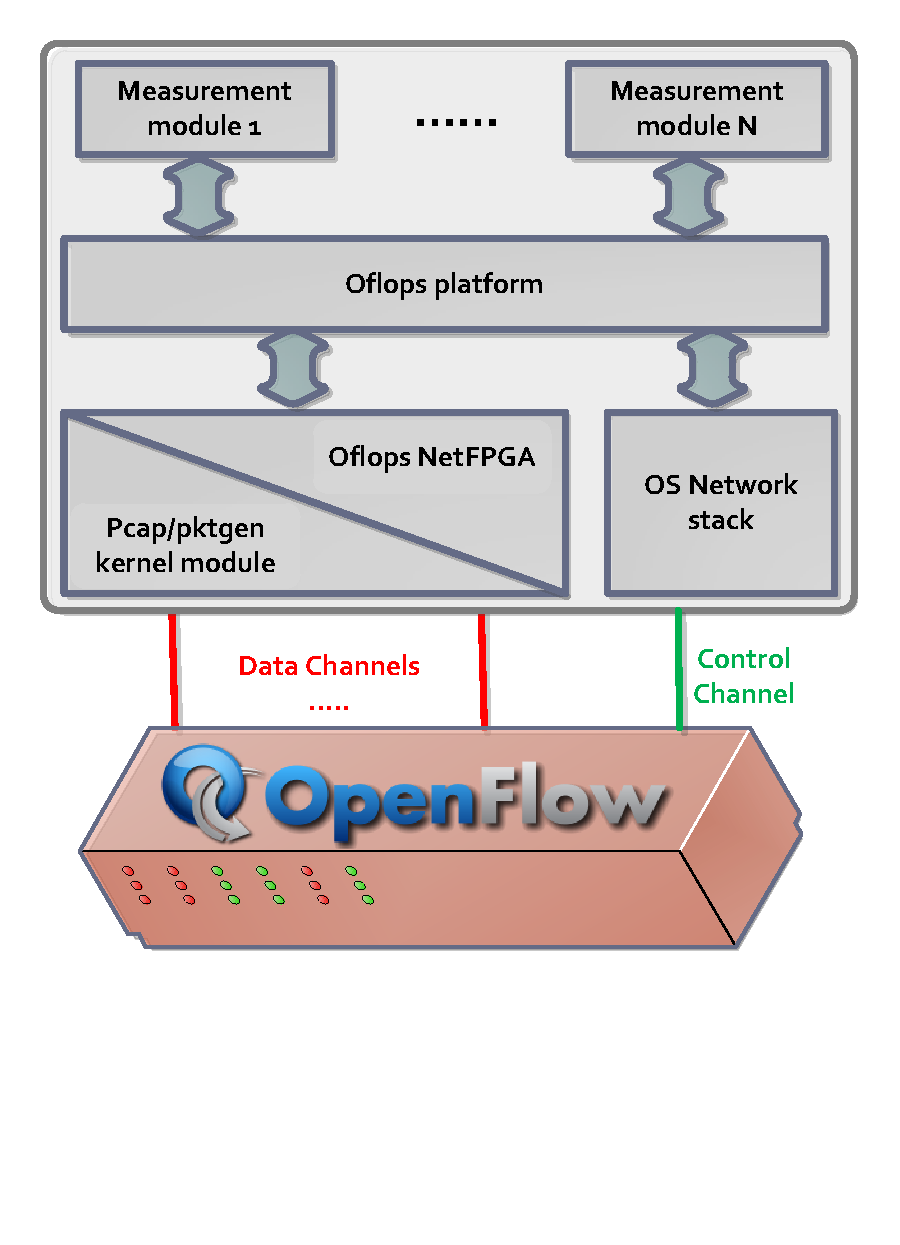
\includegraphics[width=0.99\textwidth]{openflow-design} 
\caption{\oflops design schematic}
\label{fig:oflops_design}
\end{minipage}
\begin{minipage}[b]{0.49\linewidth}
\centering
 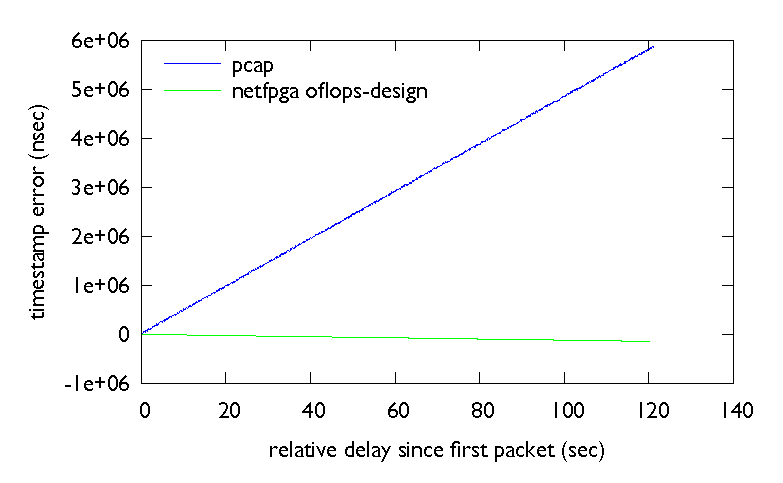
\includegraphics[width=0.99\textwidth]{timer_precision} 
 \caption{Evaluating timestamping precision using a DAG card.}
\label{fig:timestamping}
\end{minipage}
\end{figure}

The \oflops design philosophy aims to develop a low overhead abstraction layer
that allows interaction with an OpenFlow-enabled device over multiple data
channels.  The platform provides a unified system that allows developers to
control and receive information from multiple control sources: data and control
channels as well as SNMP to provide specific switch-state information.
For the development of measurement experiments over \oflops, the platform
provides a rich, event-driven, API that allows developers to handle events
programatically in order to implement and measure custom controller
functionality. The current version is written predominantly in C. Experiments
are compiled as shared libraries and loaded at run-time using a simple
configuration language, through which experimental parameters can be defined.
A schematic of the platform is presented in Figure~\ref{fig:oflops_design}.
Details of the \oflops programming model can be found in the API manual
\cite{oflops-manual}.

The platform is implemented as a multi-threaded application, to take
advantage of modern multicore environments. To reduce latency, our design
avoids concurrent access controls: we leave any concurrency-control complexity 
to individual module implementations. \oflops consists of the following five threads, 
each one serving specific type of events:\\
\textbf{1. Data Packet Generation}: control of data plane traffic generators.\\
\textbf{2. Data Packet Capture}: data plane traffic interception.\\
\textbf{3. Control Channel}: controller events dispatcher.\\
\textbf{4. SNMP Channel}: SNMP event dispatcher.\\
\textbf{5. Time Manager}: time events dispatcher.

\oflops provides the ability to control concurrently multiple data
channels to the switch. Using a tight coupling of the data and control 
channels, programers can understand the impact of the measurement
scenario on the forwarding plane. To enable our platform to run on
multiple heterogeneous platforms, we have integrated support for
multiple packet generation and capturing mechanisms. For the packet
generation functionality, \oflops supports three mechanisms:
user-space, kernel-space through the pktgen module~\cite{pktgen}, and
hardware-accelerated through an extension of the design of the NetFPGA
Stanford Packet Generator~\cite{Covington09}.  For the packet
capturing and timestamping, the platform supports both the pcap
library and the modified NetFPGA design. Each approach provides
different precisions and different impacts upon the measurement
platform.

A comparison of the precision of the traffic capturing mechanisms is 
presented in Figure~\ref{fig:timestamping}. In this experiment we 
use a constant rate 100 Mbps probe of small packets for a two minute 
period. The probe is duplicated, using an optical wiretap with negligible 
delay, and sent simultaneously to OFLOPS and to a DAG card. In the figure, 
we plot the differences of the relative timestamp between each OFLOPS 
timestamping mechanism and the DAG card for each packet. From the figure, 
we see that the pcap timestamps drift by 6 milliseconds after 2 minutes.
On the other hand, the NetFPGA timestamping mechanism has a smaller
drift at the level of a few microseconds during the same period.

% In order to present the precision of each timestamping mechanism, we
% perform a comparison against a DAG card using a 100Mbps packet probe of
% small packet for a monitoring period of 2 minutes (maximum running
% time among all current \oflops modules).  The measurement is contacted
% using an optical wire tap, ensuring traffic duplication with
% negligible delays.  The timestamp differences between each capturing
% mechanism and the dag card are plotted .  In the figure we see that the pcap
% timestamps drift by 6 milliseconds after 2 minutes.
% % while they appear spiky because the percision is on the
% %level of microsends. 
% On the other hand, the NetFPGA timestamping mechanism has a smaller
% precision error at the level of a few microseconds.
%
% \todo{steve: this is why for our purposes we want to have accuracy but we should
% be open and say that depending on the accuracy you really want, how much 
% this really is a problem}
%
% \subsection{old design}
%
%
% We have designed the \oflops\footnote{The \oflops source code is
% made available to the community under an open source license.} 
% tool to assess the performance of OpenFlow
% implementations. The \oflops design-philosophy is to permit an
% abstraction of the interaction with an OpenFlow-enabled device without
% introducing significant additional processing delays.
% % \comment{How much processing delay does \oflops introduce? Just
% %   rought numbers to give an idea...}  \comment{haris: I have this
% %   measurement. I will cover it in the testbed introduction}
% For the development of measurement experiments over \oflops, the
% platform, this version written predominantly in C, provides a rich,
% event-driven, API that allows developers to handle events
% programatically. Experiments are compiled as shared libraries and
% loaded at run-time through a configuration file. The configuration
% file allows the user to define the parameters of the experiment. A
% schematic of the platform is presented in
% Figure~\ref{fig:oflops_design}.  \todo{add a pointer to the \oflops API
%   manual in order to address the claim of how easy it is to develop
%   module for \oflops.}

% In order to assess the performance of a network device that has both
% rich functionality and for which we have little idea of the
% implementation, we require a diverse set of concurrent measurements
% able to encompass all parameters of an experiment. Furthermore,
% to achieve high accuracy across a range of control and measurement
% tasks, we designed a unified platform that permits us to obtain
% information from multiple sources: data and control channels as well
% as SNMP to provide specific switch-state information.

% An OpenFlow controller is the core component of our \oflops framework.
% While OpenFlow controllers like \cite{Gude08,SNAC} provide advanced
% APIs that support fine-grained control of the switch, they do this
% through extensions based upon language mechanisms such as C++ 
% bindings to Python. Such extensions were found to introduce poor 
% performance through added complexity on the control channel, 
% resulting in misleading measurement noise. To further reduce measurement 
% noise, the control flow is configured to provide a path with minimal 
% latency overheads (rather than ones optimised for bulk throughput).

% \oflops provides the ability to control concurrently multiple data
% channels to the switch. By embedding the data channel within the
% platform we are able to understand the impact of the measurement
% scenario on the switching plane. Wanting our platform to run on
% multiple heterogeneous platforms, we have integrated support for
% multiple packet generation and capturing mechanisms. For the packet
% generation functionality, \oflops supports three mechanisms: user-space,
% kernel-space through the pktgen module~\cite{pktgen}, and hardware-accelerated
% through a generator that extends the NetFPGA Stanford Packet
% Generator~\cite{Covington09}.  For the packet capturing and
% timestamping, the platform supports both the pcap library and a
% modified version of the packet capture-functionality from the NetFPGA
% Stanford Packet Generator design. Each approach provides different
% precisions and different impacts upon the measurement platform.
% \todo{steve: this is why for our purposes we want to have accuracy but we should 
% be open and say that depending on the accuracy you really want, how much 
% this really is a problem}

% The \oflops platform currently uses a simple packet generation
% model. Each packet is generated by selecting at random from a uniform
% distribution each value of the header fields from the set of possible
% values that the measurement module defines. The interval between probe
% packets may be selected in a similar fashion although for this paper we use 
% constant intervals. The goal of the \oflops packet generation is not to 
% reproduce the properties of real data traffic; although a module to provide 
% realistic cross-traffic has been tested. For each generated packet we define 
% a custom packet payload: a unique packet-id and a generation-timestamp. 
% By storing this information in the packet, data may be captured and processed 
% offline.

% % For this, we implemented an extra packet markup module in the Stanford Packet Generator hardware design. 

% % \comment{not sure the reader knows what a markup module is...nor how important it is to mention it.}
% % \comment{haris: I was interested to say that the default NF packet
% %   generato doesn't support this by default. I modified a bit the
% %   sentence, but if you think that it is not relevant feel free to
% %   remove it}

% The platform is implemented as a multi-threaded application, to take
% advantage of modern multicore environments. It consists of five
% threads, each one serving specific type of events. To reduce latency
% we have a design that avoids concurrent access controls: we leave any
% concurrency-control complexity to individual module implementations. 
% \oflops contains the following threads:\\
% \textbf{1. Data Packet Generation} a thread to initialize and run the packet probes.\\
% \textbf{2. Data Packet Capture} a thread to capture packets over the data channel
% and transfer them to the measurement module.\\
% \textbf{3. OpenFlow Control Channel} a thread to capture data over the
% control socket, parse their content and generate the appropriate events on the API mechanism.\\
% \textbf{4. SNMP Channel} a thread that monitors passively the SNMP
% channel and collect asynchronous SNMP replies. \\
% \textbf{5. Time Manager} a thread running a high precision event manager where modules can register 
% their own custom events.

% % \begin{enumerate}
% % \item \textit{Data Packet Generation} a thread to initialize and run the packet probes.
% % \item \textit{Data Packet Capture} a thread to capture packets over the data channel 
% % and transfer them to the measurement module.
% % \item \textit{Openflow Control Channel} a thread to capture data over the control socket,
% % parse their content and generate the appropriate events on the API mechanism.
% % \item \textit{SNMP Channel} a thread that monitors passively the SNMP channel and 
% % collect asyncronous SNMP replies.
% % \item \textit{Timer Events} thread, a high precision event thread where modules can 
% % register their own custom events.
% % \end{enumerate}

% % % \Begin{itemize}
% % \item What is the purpose
% % \item 3 threads running in parallel. Separation of task for each
% %   thread.
% % \item what changes occurred in the verilog code of the Stanford
% %   packet generator\cite{Covington09}
% % \item no other hw design provides in parallel packet generation and
% %   packet capturing in parallel.
% % \item we are kinda of during a regression suite which is there to
% %   define performance specifications.
% % \end{itemize}

\section{Measurement setup}\label{sec:oflops-switches}
%
%\todo{Make this a bit more tight to save some space. Need to explain
%why we anonymize the switches. Add a reference to table 2 explaining
%what is show there.}

The number of \of-enabled devices has slowly increased recently, with
switch and router vendors providing experimental \of support such
as prototype and evaluation firmware. At the end of 2009, the \of
protocol specification was released in its first stable version 1.0~\cite{openflow-spec}, 
the first recommended version implemented by vendors for production systems. 
Consequently, vendors did proceed on maturing their prototype implementations, 
offering production-ready \of-enabled switches today. Using \oflops, we 
evaluate \of-enabled switches from three different switch vendors.
Vendor 1 has production-ready \of support, whereas vendors 2 and
3 at this point only provide experimental \of support. 
The set of selected switches provides a representative but not
exhaustive sample of available \of-enabled top-of-rack-style
switching hardware. Details regarding the CPU and the size of the
flow table of the switches are provided in Table~\ref{tbl:switch_list}.

\of is not limited to hardware. The \of protocol reference is the software
switch, OpenVSwitch~\cite{openvswitch}, an important implementation for
production environments. Firstly, OpenVSwitch provides a replacement for the
poor-performing Linux bridge~\cite{bianco10}, a crucial functionality for
virtualised operating systems.  Secondly, several hardware switch vendors use
OpenVSwitch as the basis for the development of their own \of-enabled firmware.
OpenVSwitch development team has standardised a clean abstraction over the
control of the switch silicon (similar to linux HAL), which allows code reuse
over any forwarding entity that implements the switch abstraction. Thus, the
mature software implementation of the \of protocol is ported to commercial
hardware, making certain implementation bugs less likely to (re)appear.  In this
paper, we study OpenVSwitch alongside our performance and scalability study of
hardware switches. Finally, in our comparison we include the \of switch design
for the NetFPGA platform~\cite{openflow-netfpga}. This implementation is based
on the \of reference implementation, extending it with a hardware forwarding
design. 

\begin{table}[h!]
  \begin{center}
{
  \begin{tabular}{ |c | c | c | }
    \hline                        
    \textbf{Switch} & \textbf{CPU} & \textbf{Flow table size} \\
    \hline  
    Switch1 & PowerPC 500MHz & 3072 mixed flows \\
    \hline  
    Switch2 & PowerPC 666MHz & 1500 mixed flows \\
    \hline  
    Switch3 & PowerPC 828MHz & 2048 mixed flows \\
    \hline  
    OpenVSwitch & Xeon 3.6GHz & 1M mixed flows \\
    \hline  
    NetFPGA &  DualCore 2.4GHz & 32K exact \& 100 wildcard \\
    \hline 
  \end{tabular}  

}
\end{center}
\caption{OpenFlow switch details.}
\label{tbl:switch_list}
\end{table}

In order to conduct our measurements, we setup \oflops on a dual-core
2.4GHz Xeon server equipped with a NetFPGA card.
For all the experiments we utilize the NetFPGA-based packet generating and 
capturing mechanism. 1Gbps control and data channels are connected directly 
to the tested switches. We measure the processing delay incurred by the 
NetFPGA-based hardware design to be a near-constant $900$ nsec independent 
of the probe rate.
% In order to define any possible bias introduced by the hardware
% design, we connect two ports of the netfpga card and generate a high
% rate packet probe of small packet. By comparing the generation and
% capture timestamps provided by the platform we measure the delay to
% be constant at 900 nanoseconds.
% This entity contains descriptions of flows, based on the field of
% the openflow tupple, and the actions applied over each matched
% packet. In any openflow-enabled switch there can be numerous flow
% tables with each table having different capabilities. As a general
% rule of thumb, Openflow implementations contain a large software
% table stored in main memory, capable of switching packets at low
% rates, and a smaller h/w based or kernel space table, capable to
% support high rate switching. So far, protocol specifications don't
% define how the switch is expected to allocate flows in flow tables
% and this has led to a diverse set of approaches. Ultimately, the
% goal for an openflow baed application is to keep its large volume
% flows on the fast flow table. Using \oflops we were interested to
% quantify 2 things: the impact of flow manipulation algorithms on the
% switching plane and the scaling properties of the table manipulation
% mechanism. Both of this delays are important when a system has to
% In order to present the capabilities of our tool we develop a set of
% simple experiments using the \oflops platform in order to benchmark
% the perfomance of some simple use case scenarios of the
% protocol. The results of this experiments are presented later in
% Scetion \ref{sec:result}. For our experiment we use four openflow
% implementations which cover a diverse set from available
% implementations. The details of the implementations under test can
% be found in table \ref{tbl:switch_list}. Switch1 and Switch2 are
% hardware switches that support the openflow protocol in their
% firmware. \oflops is installed on a 4 core Intel Xeon server with a
% NetFPGA card. For each switch we connect one of the ports to a
% commodity NIC port of the server, in order to use it as the control
% channel, and 4 other ports to the 4 ports of the NetFPGA card, in
% order to use them as the data channels.
% An important aspect that we noticed during experimentation is the
% fundamental limits that software switches face regarding switching
% performance. Specifically, software switches implement all their
% functionality in the CPU. Because of this, in order for the switch
% to decide the output port for each packet, it has to copy the whole
% packet in main memory. Unfortunately, motherboard buses have limited
% capacity and this may result in packet queueing when the packet rate
% increases. The results of this problem is illustrated in
% Figure~\ref{fig:switch_delay}. In this experiment we are sending a
% single packet probe of small packets and measure the median RTT when
% we increase the packet rate. In the Figure we can see that software
% switches introduce buffering delay on the probe when the packet rate
% icnreases, while hardware accelerated switches can switch packets at
% line rate. Because of this effect we are concious to restrict all
% measurement probes at rates that will not introduce bias during
% comparison.
% \begin{figure}[htb]
%   \begin{center}
%     \includegraphics[width=0.4\textwidth]{graphs/switch_delay/switch-delay}
%   \end{center}
%   \caption{switching delay of implementations}
%   \label{fig:switch_delay}
% \end{figure}
%
% LocalWords: defacto facto virtualised OpenVSwitch Xeon GHz Gb
% NetFPGA Oflops LocalWords: DualCore PowerPC OpenFlow IP VMs


%%%%%%%%%%%%%%%%%%%%%%%%%%%%%%%%%%%%%%%%%%%%%%%
\section{Switch Evaluation}\label{sec:oflops-result}
%%%%%%%%%%%%%%%%%%%%%%%%%%%%%%%%%%%%%%%%%%%%%%%%

% In this section we present a set of tests performed by \oflops to
% measure the behavior and performance of \of-enabled
% devices. These tests target (1) the \of packet processing 
% actions, (2) the update rate of the \of flow table along with 
% its impact on the data plane, (3) the monitoring capabilities provided 
% by \of, and (4) the impact of interactions between different 
% \of operations.

As for most networking standards, there are different ways to implement a
given protocol based on a paper specification. \of is not different in this
regard. The current reference implementation is defined through OpenVSwitch
\cite{openvswitch}. However, different software and hardware implementations may
not implement all features defined in the OpenVSwitch reference, or they may
behave in an unexpected way. In order to understand the behaviour of switch \of
implementation, we develop a suite of measurement experiments to
benchmark the functionality of the elementary protocol interactions.  These
tests target (1) the \of packet processing actions~\ref{sec:result-packets}, (2)
the packet interception and packet injection functionality of the
protocol~\ref{sec:result-pktin}, (3) the update rate of the \of flow table along
with its impact on the data plane,~\ref{sec:result-rate} (4) the monitoring
capabilities provided by \of, and (5) the impact of interactions between
different \of operations.


%As for most networking standards, there are different ways of implementing 
%a given protocol based on a paper specification. OpenFlow is not different in 
%this regard. The current reference implementation is defined through
%OpenVSwitch \cite{openvswitch}. However, different software and hardware
%implementations may not implement all features defined in the
%OpenVSwitch reference, or they may behave in an unexpected way. We
%therefore propose two types of tests within \oflops: feature-oriented
%and performance-oriented. Feature-oriented tests verify which types
%of OpenFlow messages are supported by a given implementation.
%Performance-oriented tests aim to reveal not only the raw performance
%delivered by a given OpenFlow implementation, but also subtle
%interactions between the OpenFlow control plane and the data plane, or
%between different parts of the OpenFlow control plane.

\subsection{Packet modifications}\label{sec:results-packets}

The \of specification \cite{openflow-spec} defines ten packet
modification actions which can be applied on incoming
packets. Available actions include modification of MAC, IP, and VLAN
values, as well as transport-layer fields. A flow definition can
contain any combination of them. The left column of
Table~\ref{tbl:feature_delay} lists the packet fields that can be
modified by an \of-enabled switch.
These actions are used by network devices such as IP routers (e.g.,
rewriting of source and destination MAC addresses) and NAT (rewriting
of IP addresses and ports). Existing network equipment is tailored to
perform a subset of these operations, usually in hardware to sustain
line rate. On the other hand, how these operations are to be used is
yet to be defined for new network primitives and applications, such as
network virtualization, mobility support, or flow-based traffic
engineering.

% Explain how we measure the time taken to perform the modification.
To measure the time taken by an OpenFlow implementation to modify a
packet field header, we generate from the NetFPGA card UDP packets of
100 bytes at a constant rate of 100Mbps (approx. 125 Kpps). 
This rate is high enough to give statistically significant results in
a short period of time, without causing any packet queuing for any of the
switches.  The flow table is initialized with a flow that
applies a specific action on all probe packets and the processing
delay is calculated using the transmission and receipt timestamps,
provided by the NetFPGA.
%, while also low enough so that the impact of
%queuing at the network interface cards can be ignored. 
%Each packet is
%timestamped when leaving the NetFPGA card. The packet then arrives at
%the OpenFlow switch via a direct 1Gbps Ethernet link, the switch
%matches the packet against the flow table, and sends it back to the
%NetFPGA card where it is timestamped again.

\begin{table*}[tb]
\begin{flushleft}
        \begin{tabular}[t]{ |l | c | c | c || c | c | c  || c | c | c | }
          \hline                       
          Mod. type & \multicolumn{3}{|c|}{Switch 1} & \multicolumn{3}{|c|}{ovs} &
          \multicolumn{3}{|c|}{Switch 2} \\ 
          \hline                       
          & med & sd & loss\%  & med & sd & loss\% & med & sd & loss\%\\
          \hline  
          Forward & 4 & 0 & 0 & 35 & 13 & 0& 6 & 0 & 0 \\
          \hline  
          MAC addr. & 4 & 0 & 0 & 35 & 13 & 0& 302 & 727 & 88\\
          \hline  
          IP addr. & 3 & 0 & 0 & 36 & 13 & 0 & 302 & 615 & 88\\
          \hline  
          IP ToS & 3 & 0 & 0 & 36 & 16 & 0 & 6 & 0 & 0\\
          \hline  
          L4 port & 3 & 0 & 0 & 35 & 15 & 0 & 302 & 611 &  88\\
          \hline  
          VLAN pcp & 3 & 0 & 0 & 36 & 20 & 0 & 6 & 0 & 0\\
          \hline  
          VLAN id & 4 & 0 & 0 & 35 & 17 & 0 & 301 & 610 & 88\\
          \hline  
          VLAN rem. & 4 & 0 & 0 & 35 & 15 & 0 & 335 & 626 & 88\\
      \hline
    \end{tabular}
   \begin{tabular}[t]{ |l | c | c | c || c | c | c | }
          \hline                       
          Mod. type & \multicolumn{3}{|c|}{Switch 3} & \multicolumn{3}{|c|}{NetFPGA}\\ 
          \hline                       
          & med & sd & loss\%  & med & sd & loss\% \\
          \hline  
          Forward & 5 & 0 & 0 & 3 & 0 & 0 \\
          \hline  
          MAC addr. & - & - & 100 & 3 & 0 & 0 \\
          \hline  
          IP addr. & - & - &  100 & 3 & 0 & 0 \\
          \hline  
          IP ToS & - & - & 100 & 3 & 0 & 0 \\
          \hline  
          L4 port & - & - & 100 & 3 & 0 & 0 \\
          \hline  
          VLAN pcp & 5 & 0 & 0 & 3 & 0 & 0 \\
          \hline  
          VLAN id & 5 & 0 & 0 & 3 & 0 & 0  \\
          \hline  
          VLAN rem. & 5 & 0 & 0 & 3 & 0 & 0 \\
      \hline
    \end{tabular}
 
\caption{Time in $\mu$s to perform individual packet modifications and packet
loss. Processing delay indicates whether the operation is
  implemented in hardware (\textless10$\mu$s) or performed by the CPU (\textgreater10$\mu$s).}
  \label{tbl:feature_delay}
\end{flushleft}
\end{table*}
% What the table shows...
Evaluating individual packet field modification,
Table~\ref{tbl:feature_delay} reports the median difference between
the generation and capture timestamp of the measurement probe along
with its standard deviation and percent of lost packets.

We observe significant differences in the performance of the hardware
switches due in part to the way each handles packet
modifications. Switch1, with its production-grade implementation,
handles all modifications in hardware; this explains its low packet
processing delay between 3 and 4 microseconds. On the other hand,
Switch2 and Switch3 each run experimental firmware providing only
partial hardware support for \of actions. Switch2 uses the switch
CPU to perform some of the available field modifications, resulting in two orders
of magnitude higher packet processing delay and variance.
Switch3 follows a different approach: All packets of flows with
actions not supported in hardware are silently discarded. The
performance of the OpenVSwitch software implementation lies between
Switch1 and the other hardware switches.  OpenVSwitch fully implements
all \of actions. However, hardware switches outperform
OpenVSwitch when the flow actions are supported in hardware.
% than the delay of the hardware path of the hardware switches,
% dominated by the NIC-CPU latency.
%
% For example, the time of an ensemble of modifications is dictated by the
% maximum time across all modifications.\todo{Last sentence is reported to be
% misleading by the reviewers}
% Furthermore, we notice that for switch1 and openvswitch there is
% limit of 7 actions, which may enveil similrities in the code base.
% From the results presented in Table~\ref{tbl:feature_delay}, we can
% already conclude that an experimental hardware-based OpenFlow
% implementation is likely to deliver poor performance compared to a
% mature software-based implementation running on commodity PC
% hardware

We conducted a further series of experiments with variable numbers of packet
modifications as flow actions. We observed, that the combined processing time of
a set of packet modifications is equal to the highest processing time across all
individual actions in the set. Furthermore, we notice that for Switch1 and 
OpenVSwitch there is a limit of 7 actions, which potentially exposes some
relation in the code base.

\subsection{Traffic interception and injection}\label{sec:results-pktin}

\begin{figure}[ht]
  \begin{center}
    \subfigure[Packet in message latency]
    {\includegraphics[width=0.99\textwidth]{pkt_in_delay}}
    \subfigure[Packet out message latenct]
	{\includegraphics[width=0.99\textwidth]{pkt_out_delay}}
  \end{center}
  \caption{Latency to intercept or inject a packet using the \of protocol}
  \label{fig:pkt_in_out_delay}
\end{figure}

\of protocol permits a controller to intercept or inject traffic over the
control plane. This functionality allowed in the initial design of the \of
controller to be reactive and handle traffic on a per-flow basis. Packet
injection allows the controller to interact with connected network hosts. The
interception mechanism in \of has been reported in the initials deployments of
the protocol to cause significant slow-down in the control plane and led to
switch disconnection at high data rate~\cite{Kobayashi:vn}. This is a direct
consequence of the silicon design in current \of switches, that develop such
functionality as an low-frequency exception mechanism. In order to characterise
this functionality, we develop a simple experiment using \oflops that sends
packets at a specific rate and measure the latency of the switch to process
them. In Figure~\cite{fig:pkt_in_out_delay}, we show the latency induced on
packets both for Packet\_in and Packet\_out messages. We omit in this experiment
Switch 3 as this functionality maxed out its CPU utilisation and after a few seconds
made the switch unresponsive over the control channel. For packet\_out messages,
the switches rate limit through the tcp connection channel the rate of messages
received and as a result they provide a constant performance. For packet\_in
messages, we observe a diverse behaviour between hardware switches at high
packet rates. For Switch 1, packet loss and latency gets high for traffic rates 
above 400 packets per second. Additionally, we noticed that the switch is able to 
process a maximum of 500 packets/sec. For Switch 2 latency and packet loss are 
significantly lower and stable. Switch 2 faced problem to process packet  
important packet at high rates of 2000 packets per second. OpenVSwitch, has a high 
but stable latency for any tested data rates. 

\subsection{Flow table update rate}\label{sec:results-rate}

% So far, we get packet modification primitives and the expected performance that software/hardware can/should deliver.
% 
\begin{figure}[ht]
  \begin{center}
    \subfigure[OpenVSwitch (log-log scale)]
    {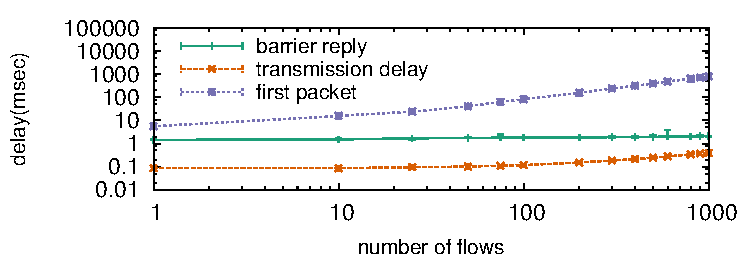
\includegraphics[width=0.99\textwidth]{openvswitch_mod_flow_exact_comparison}}
    \subfigure[Switch1 (log-log scale)]
	{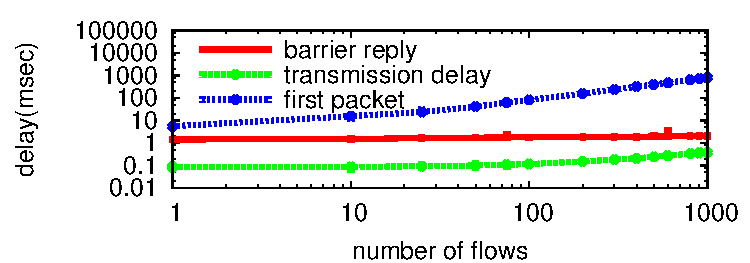
\includegraphics[width=0.99\textwidth]{nec_mod_flow_exact_comparison}}
  \end{center}
  \caption{Flow entry insertion delay: as reported using the
    \texttt{barrier} notification and as observed at the data
    plane.}
  \label{fig:flow_insertion_comparison}
\end{figure}

The flow table is a central component of an OpenFlow switch and is the
equivalent of a Forwarding Information Base (FIB) on routers. Given the
importance of FIB updates on commercial routers, e.g., to reduce the impact of
control plane dynamics on the data plane, the FIB update processing time of
commercial routers provide useful reference points and lower bounds for the time
to update a flow entry on an OpenFlow switch. The time to install a new entry on
commercial routers has been reported in the range of a few hundreds of
microseconds~\cite{shaikh-igp}.

OpenFlow provides a mechanism to define barriers between sets of
commands: the \texttt{barrier} command. According to the OpenFlow
specification~\cite{openflow-spec}, the barrier command is a way to be
notified that a set of OpenFlow operations has been completed. Further, 
the switch has to complete the set of operations issued prior to the barrier 
before executing any further operation. If the OpenFlow implementations 
comply with the specification, we expect to receive a barrier notification for 
a flow modification once the flow table of the switch has been updated, 
implying that the change can be seen from the data plane.

We check the behavior of the tested OpenFlow implementations,
finding variation among them. For OpenVSwitch and Switch1,
Figure~\ref{fig:flow_insertion_comparison} shows the time to install a
set of entries in the flow table. The NetFPGA-based switch results
(not reported) are similar to those of Switch1, while Switch2 and Switch3 
are not reported as this OpenFlow message is not supported by the firmware. 
For this experiment, \oflops relies on a stream of packets of 100 bytes at
a constant rate of 10Mbps that targets the newly installed flows in a
round-robin manner. The probe achieves sufficiently low inter-packet
periods in order to measure accurately the flow insertion time.
%With such a probe stream, we obtain an inter-packet
%period of less than 100$\mu$s, adequate for measuring any change in
%the flow-insertion time.

In Figure~\ref{fig:flow_insertion_comparison}, we show three different
times. The first, {\it barrier notification}, is derived by measuring the time 
between when the \textbf{first insertion command} is sent by the \oflops 
controller and the time the barrier notification is received by the PC. The 
second, {\it transmission delay}, is the time between the first and 
last flow insertion commands are sent out from the PC running \oflops. 
The third, {\it first packet}, is the time between the \textbf{first insertion
 command} is issued and a packet has been observed for the last of
the (newly) inserted rules. For each configuration, we run the
experiment 100 times and Figure~\ref{fig:flow_insertion_comparison}
shows the median result as well as the $10^{th}$ and $90^{th}$ percentiles 
(variations are small and cannot be easily viewed).
%\todo{point that the error
%  bounds are tight and cannot easily viewed on the graph}

From Figure~\ref{fig:flow_insertion_comparison}, we observe that even
though the {\it transmission delay} for sending flow insertion commands 
increases with their number, this time is negligible when compared with 
data plane measurements ({\it first packet}). Notably, the {\it barrier notification} 
measurements are almost constant, increasing only as the transmission delay 
increases (difficult to discern on the log-log plot) and, critically, this operation 
returns before any {\it first packet} measurement. This implies that the way
the {\it barrier notification} is implemented does not reflect the time when 
the hardware flow-table has been updated.

In these results we demonstrate how \oflops can compute per-flow
overheads. We observe that the flow insertion time for Switch1
starts at $1.8$ms for a single entry, but converges toward an
approximate overhead of $1$ms per inserted entry as the number of
insertions grows.

%%%%%%%%%%%%%%%%%%%%%%%%%%%%%%%%%%%%%%%%%%%%%%
\subsubsection*{Flow insertion types}
%%%%%%%%%%%%%%%%%%%%%%%%%%%%%%%%%%%%%%%%%%%%%%

\begin{figure}[h]
  \begin{center}
    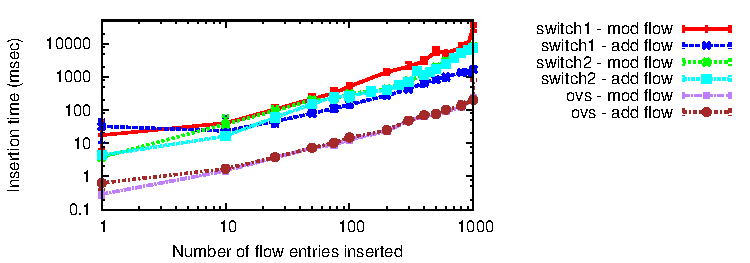
\includegraphics[width=0.80\textwidth]{flow_insertion_delay}
  \end{center}
  \caption{Delay of flow insertion and flow modification, as observed
    from the data plane (log-log scale).}
  \label{fig:flow_insertion_delay}
\end{figure}

We now distinguish between flow insertions and the modification of existing flows.  
With OpenFlow, a flow rule may perform exact packet matches or use wild-cards to 
match a range of values. Figure~\ref{fig:flow_insertion_delay} compares the flow
insertion delay as a function of the number of inserted entries. This is done for the 
insertion of new entries and for the modification of existing entries.

These results show that for software switches that keep all entries in memory, the 
type of entry or insertion does not make a difference in the flow insertion time.
Surprisingly, both Switch1 and Switch2 take more time to modify existing flow entries 
compared to adding new flow entries.  For Switch1, this occurs for more than 10 new 
entries, while for Switch2 this occurs after a few tens of new entries.
After discussing this issue with the vendor of Switch2, we came to the
following conclusion: as the number of TCAM entries increases, updates
become more complex as they typically requires re-ordering of existing
entries.

Clearly, the results depend both on the entry type and implementation.
For example, exact match entries may be handled through a hardware or
software hash table. Whereas, wild-carded entries, requiring support
for variable length lookup, must be handled by specialized memory
modules, such as TCAM. With such possible choices and range of
different experiments, the flow insertion times reported in
Figure~\ref{fig:flow_insertion_delay} are not generalizable, but
rather depend on the type of insertion entry and implementation.

% %%%%%%%%%%%%%%%%%%%%%%%%%%%
\subsection{Flow monitoring}\label{sec:results-monitoring}
% %%%%%%%%%%%%%%%%%%%%%%%%%%%

The use of OpenFlow as a monitoring platform has already been
suggested for the applications of traffic matrix
computation~\cite{opentm-pam,tm-presto} and identifying large traffic
aggregates~\cite{openflow-measurement-hotice}. To obtain direct
information about the state of the traffic received by an OpenFlow
switch, the OpenFlow protocol provides a mechanism to query traffic
statistics, either on a per-flow basis or across aggregates matching
multiple flows and supports packet and byte counters. 
%The result of a query returns packet and byte
%counters, either for the matched flows individually or for the
%aggregate.

We now test the performance implications of the traffic statistics reporting 
mechanism of OpenFlow. Using \oflops, we install flow entries that match 
packets sent on the data path. Simultaneously, we start sending flow statistics 
requests to the switch. Throughout the experiment we record: the delay getting 
a reply for each query, the amount of packets that the switch sends for each 
reply and the departure and arrival timestamps of the probe packets.

Figure~\ref{fig:stat_request} reports the time to receive a flow
statistics reply for each switch, as a function of the request
rate. Despite the rate of statistics requests being modest, quite high
CPU utilization results for even a few queries per second being
sent. Figure~\ref{fig:stat_request} reports the switch-CPU utilization
as a function of the flow statistics inter-request time. Statistics
are retrieved using SNMP. Switch3 is excluded for lack of SNMP
support.

\begin{figure}[h]
  \begin{center}
    \subfigure[Reply time.]
    {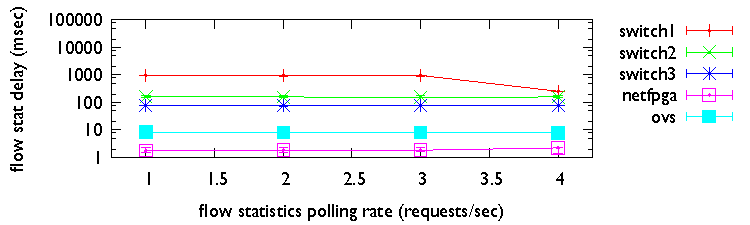
\includegraphics[width=0.99\textwidth]{flow_stats_delay}}
    \subfigure[CPU utilization.]
      {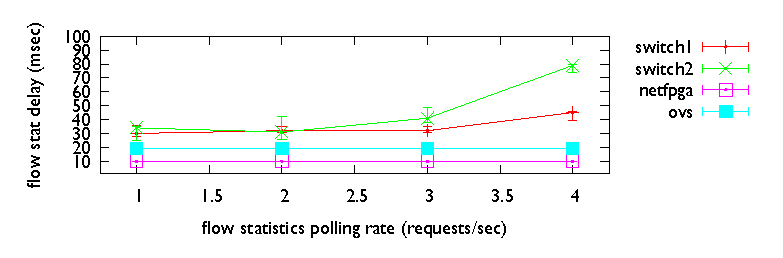
\includegraphics[width=0.99\textwidth]{flow_stats_cpu}\label{fig:stat_request_cpu}}
  \end{center}
  \caption{Time to receive a flow statistic (median) and corresponding CPU utilization.}
  \label{fig:stat_request}
\end{figure}

From the flow statistics reply times, we observe that all switches have (near-)constant 
response delays: the delay itself relates to the type of switch.
As expected, software switches have faster response times than
hardware switches, reflecting the availability of the information in memory
without the need to poll multiple hardware counters. These consistent response
times also hide the behavior of the exclusively hardware switches
whose CPU time increases proportionally with the rate of requests.  We
observe two types of behavior from the hardware switches: the switch
has a high CPU utilization, answering flow-stats requests as fast as
possible (Switch2), or the switch delays responses, avoiding
over-loading its CPU (Switch1). Furthermore, for Switch1,
we notice that the switch is applying a pacing mechanism on its
replies. Specifically, at low polling rates the switch splits its
answer across multiple TCP segments: each segment containing statistics for a
single flow.  As the probing rate increases, the switch
will aggregate multiple flows into a single segment. This suggests that 
independent queuing mechanisms are used for handling flow statistics 
requests. Finally, neither software nor NetFPGA switches see an 
impact of the flow-stats rate on their CPU, thanks to their significantly 
more powerful PC CPUs (Table~\ref{tbl:switch_list}).

%%%%%%%%%%%%%%%%%%%%%%%%%%%%%%%%%%%%%%%%%
\subsection{OpenFlow command interaction}\label{sec:results-interactions}
%%%%%%%%%%%%%%%%%%%%%%%%%%%%%%%%%%%%%%%%%

% why is it important this experiment

An advanced feature of the OpenFlow protocol is its ability to
provide applications with, e.g., flow arrival notifications from the 
network, while simultaneously providing fine-grain control of 
the forwarding process. This permits applications to adapt
in real time to the requirements and load of the
network~\cite{plug_n_serv,Yap09}. Under certain OpenFlow usage
scenarios, e.g., the simultaneous querying of traffic statistics and
modification of the flow table, understanding the behavior of the data
and control plane of OpenFlow switches is difficult without advanced
measurement instrumentation such as the one provided by \oflops. 
%One 
%of the strengths of \oflops is that is enables the development of custom scenarios
%that stress specific aspects of the OpenFlow control or data path.

Through this scenario, we extend Section~\ref{sec:results-rate} to show 
how the mechanisms of traffic statistics extraction and table manipulation 
may interact. Specifically, we initialize the flow table with 1024 exact
match flows and measure the delay to update a subset of 100 flows. 
Simultaneously, the measurement module polls the switch for full table 
statistics at a constant rate. The experiment uses a constant rate 10Mbps 
packet probe to monitor the data path, and polls every 10 seconds for SNMP 
CPU values.

\begin{figure}[t!!]
  \begin{center}
    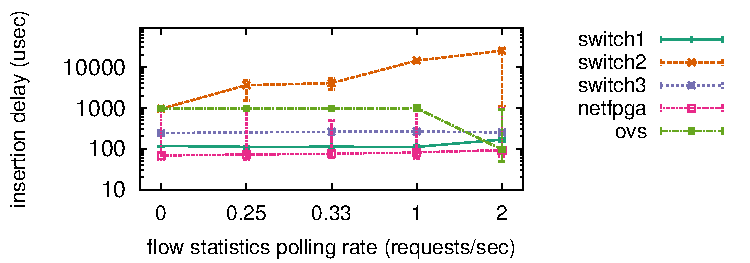
\includegraphics[width=0.99\textwidth]{interaction_test}
  \end{center}
  \caption{Delay when updating  flow table while the controller polls
    for statistics.}
  \label{fig:interaction_test}
\end{figure}

In this experiment, we control the probing rate for the flow statistics 
extraction mechanism, and we plot the time necessary for the modified 
flows to become active in the flow table. For each probing rate, we
repeat the experiment 50 times, plotting the median, $10^{th}$ and 
$90^{th}$ percentile. In Figure~\ref{fig:interaction_test} we can see
that, for lower polling rates, implementations have a near-constant
insertion delay comparable to the results of Section~\ref{sec:results-rate}.
For higher probing rates on the other hand, Switch1 and Switch3 do 
not differ much in their behavior. In contrast, Switch2 exhibits a noteworthy 
increase in the insertion delay explained by the CPU utilization increase
incurred by the flow statistics polling (Figure~\ref{fig:stat_request_cpu}). Finally,
OpenVSwitch exhibits a marginal decrease in the median insertion delay
and at the same time an increase in its variance. We believe this behavior 
is caused by interactions with the OS scheduling mechanism: the constant 
polling causes frequent interrupts for the user-space daemon of the switch, 
which leads to a batched handling of requests.

% \subsection{Timer precision} As part of each flow modification the
% protocol defines that the controller is able to define an expiration
% value for the flow. When a flow is expired, it is removed from the
% table. The protocol supports two different mechanism to define the
% timeout of a flow. Timeouts can be defined either based on the
% insertion time or the last time that the flow was used. The
% definition of the precision of this mechanism would be beneficial to
% applications that require high precision from the routing mechanism.
% In order to address the precision of the mechanism we are developing
% an experiment over the \oflops platform. The experiment utilizes 2
% ports of the switch and a single measurement probe with constant all
% field and random destination IP. During initialization the switch is
% initialized with a single wildcard flow that output packets to port
% 2. At time t=10 sec since the start of the experiment the controller
% sends an ensemble of exact match rules with different destination
% IP's and a hard expiration delay of 10 seconds. All the flows of the
% ensemble contain a single action which outputs packets on port
% 1. The experiments terminate when we receive all the flow expiration
% messages from the switch. During the experiment we log for each flow
% the time at which we received the first and last packet of the
% measurement probe for each destination IP. In the experiment we
% export as a parameter the number of flows send to the switch. For
% each number of flows we rerun the experiment for 20 times. In Figure
% \ref{fig:timer_precision} we present the results of our
% experiment. For each number of flows we plot an errorbar with the
% minimum, maximum and medium of the maximum error in the timeout of a
% flow based on the results of the packet timestamps of the
% measurement probe.
% \subsubsection*{Results}
% \subsection{Simulating a reactive switch} Simulate a Nox like
% behaviour and measure the time send at each stage of the flow
% insertion process. export as parameters the rate we send packets and
% the number of flows inserted.
% \subsubsection*{Results}
% LocalWords:  OpenFlow Oflops IP VLAN balancers SDNs virtualization NetFPGA th
% LocalWords:  UDP Mbps Gbps multiport timestamp OpenVSwitch dev dest src addr

% LocalWords:  NIC ToS TCP pcp interpacket TCAM lookup SNMP CPUs parameterising

\section{\sdnsim introduction} \label{sec:sdnsim-intro}

\section{\sdnsim design} \label{sec:sdnsim-design}

\section{\sdnsim evaluation} \label{sec:sdnsim-precision}

\subsection{\of library performance}

% In this experiment we are considering a usage scenario which queries
% the switch for unique flow statistics and modifies entries in the
% flow table. The experiment we develop is similar to the flow
% modification experiment presented in Section~\ref{sec:results-rate}.
% two packet probe streams with 100 bytes packets at a rate of
% 100Mbps.  Both probes send small packets of 100 bytes at a rate of
% 10Mbps to the switch. The first probe uses the first 100 flows of
% the table to switch packet in a round-robin manner, while the second
% probe generates packets that use randomly the rest of the flows.  At
% the same time, the controller is polling periodically the switch for
% flow statistics for variable subsets of the flow table. We also poll
% the CPU switch utilization through SNMP.  Each request queries for a
% subset of 128 flows of the table.  The controller, after one minute
% of operation, sends an ensemble of 100 flow modifications that
% change the output port of the first 100 flows of the table.  In this
% epxeriment we measure the delay between the time we send a the flow
% modification and the timer we receive at least one packet from each
% of the first 100 flows on the new port. For the duration of the
% experiment we are also polling the switches for cpu statistics.

% \subsection{Traffic interception by the controller} Because in
% Openflow the controller should be able to have full control of the
% traffic, the protocol defines a set of messages that allow the
% controller to intercept or inject traffic. In order to achieve this,
% the protocol defines 2 messages name \textit{Pkt\_in} and
% \textit{Pkt\_out}.  Pkt\_in messages are generated automatically
% when the switch has no rule to match a packet. Additionally, the
% controller is able to insert flows in the flow table that define as
% an action to push packets to the controller as pkt\_in
% messages. Each packet contains openflow specific details for the
% packet and optionally a buffer id that can be used in flow
% modification messages to push packet on a specific port
% later. Pkt\_out messages are generated by the controller and
% contains the full content of a packet and detail of how the switch
% should handle the packet.  Although these types of messages can be
% useful to openflow application developers, we need to define whether
% their limitations and the impact they have on the usage of the
% switch. In order to measure this we conduct 2 experiments. For the
% case of Pkt\_in messages we use only a single port from the switch
% on which we send a single probe with random destination IP. The rate
% of the measurement probe and the packet size are exported as
% parameters of the experiment. Before the start of the experiment we
% send a single delete message in order to clear the flow table. For
% each pkt\_in event we store its sequence number and its delay. For
% the case of Pkt\_out message we implement the reverse process. We
% generate the same measurement probe but from the controller side,
% exporting the same experiment parameters. Each packet is send on a
% specific port where it is captured by the NetFPGA card. For each
% packet we store its sequence number and its delay.
% \subsubsection*{Results}
% \begin{figure}[htb]
%   \begin{center}
%     \includegraphics[width=0.4\textwidth]{graphs/pkt_in_out/pkt_in_delay}
%   \end{center}
%   \caption{median delay to receive a pkt\_in message from the
%     switch.}
%   \label{fig:pkt_in}
% \end{figure}
% \begin{figure}[htb]
%   \begin{center}
%     \includegraphics[width=0.4\textwidth]{graphs/pkt_in_out/pkt_out_delay}
%   \end{center}
%   \caption{median delay to receive a pkt\_out message from the
%     switch.}
%   \label{fig:pkt_out}
% \end{figure}
% \begin{itemize}
% \item Nec cannot generate packet\_in packets while for packet\_out
%   after the first request the switch tears down the TCP connection
%   with an RST.
% \end{itemize}
c In this experiment we are considering a usage scenario which queries
% the switch for unique flow statistics and modifies entries in the
% flow table. The experiment we develop is similar to the flow
% modification experiment presented in Section~\ref{sec:results-rate}.
% two packet probe streams with 100 bytes packets at a rate of
% 100Mbps.  Both probes send small packets of 100 bytes at a rate of
% 10Mbps to the switch. The first probe uses the first 100 flows of
% the table to switch packet in a round-robin manner, while the second
% probe generates packets that use randomly the rest of the flows.  At
% the same time, the controller is polling periodically the switch for
% flow statistics for variable subsets of the flow table. We also poll
% the CPU switch utilization through SNMP.  Each request queries for a
% subset of 128 flows of the table.  The controller, after one minute
% of operation, sends an ensemble of 100 flow modifications that
% change the output port of the first 100 flows of the table.  In this
% epxeriment we measure the delay between the time we send a the flow
% modification and the timer we receive at least one packet from each
% of the first 100 flows on the new port. For the duration of the
% experiment we are also polling the switches for cpu statistics.

% \subsection{Traffic interception by the controller} Because in
% Openflow the controller should be able to have full control of the
% traffic, the protocol defines a set of messages that allow the
% controller to intercept or inject traffic. In order to achieve this,
% the protocol defines 2 messages name \textit{Pkt\_in} and
% \textit{Pkt\_out}.  Pkt\_in messages are generated automatically
% when the switch has no rule to match a packet. Additionally, the
% controller is able to insert flows in the flow table that define as
% an action to push packets to the controller as pkt\_in
% messages. Each packet contains openflow specific details for the
% packet and optionally a buffer id that can be used in flow
% modification messages to push packet on a specific port
% later. Pkt\_out messages are generated by the controller and
% contains the full content of a packet and detail of how the switch
% should handle the packet.  Although these types of messages can be
% useful to openflow application developers, we need to define whether
% their limitations and the impact they have on the usage of the
% switch. In order to measure this we conduct 2 experiments. For the
% case of Pkt\_in messages we use only a single port from the switch
% on which we send a single probe with random destination IP. The rate
% of the measurement probe and the packet size are exported as
% parameters of the experiment. Before the start of the experiment we
% send a single delete message in order to clear the flow table. For
% each pkt\_in event we store its sequence number and its delay. For
% the case of Pkt\_out message we implement the reverse process. We
% generate the same measurement probe but from the controller side,
% exporting the same experiment parameters. Each packet is send on a
% specific port where it is captured by the NetFPGA card. For each
% packet we store its sequence number and its delay.
% \subsubsection*{Results}
% \begin{figure}[htb]
%   \begin{center}
%     \includegraphics[width=0.4\textwidth]{graphs/pkt_in_out/pkt_in_delay}
%   \end{center}
%   \caption{median delay to receive a pkt\_in message from the
%     switch.}
%   \label{fig:pkt_in}
% \end{figure}
% \begin{figure}[htb]
%   \begin{center}
%     \includegraphics[width=0.4\textwidth]{graphs/pkt_in_out/pkt_out_delay}
%   \end{center}
%   \caption{median delay to receive a pkt\_out message from the
%     switch.}
%   \label{fig:pkt_out}
% \end{figure}
% \begin{itemize}
% \item Nec cannot generate packet\_in packets while for packet\_out
%   after the first request the switch tears down the TCP connection
%   with an RST.
% \end{itemize}
\subsection{NS-3 performance}

\section{Security Tradeoffs on Datacenter Network Micro-control} \label{sec:rdsf-eval}

%%%%%%%%%%%%%%%%%%%%%%%%%%%%%%
\section{Summary and Conclusions}\label{sec:conclusion}
%%%%%%%%%%%%%%%%%%%%%%%%%%%%%%
  
We presented, \oflops, a tool that tests the capabilities and performance of 
OpenFlow-enabled software and hardware switches. \oflops combines advanced 
hardware instrumentation, for accuracy and performance, and provides an extensible 
software framework. We use \oflops to evaluate five different OpenFlow switch 
implementations, in terms of OpenFlow protocol support as well as performance.
%In our performance evaluation, we benchmark the packet processing, flow table
%modification and traffic statistics export functionalities of the switches.

We identify considerable variation among the tested OpenFlow implementations.
We take advantage of the ability of \oflops for data plane measurements to
quantify accurately how fast switches process and apply OpenFlow commands.
For example, we found that the barrier reply message is not correctly implemented,
making it difficult to predict when flow operations will be seen by the data plane.
Finally, we found that the monitoring capabilities of existing hardware switches 
have limitations in their ability to sustain high rates of requests. Further, at high 
rates, monitoring operations impact other OpenFlow commands.

We hope that the use of \oflops will trigger improvements in the
OpenFlow protocol as well as its implementations by various vendors.

%We also readily acknowledge this paper as a snapshot of work in
%progress; every set of results poses new questions but also the role
%of \oflops can evolve as new OpenFlow instantiations are introduced and
%existing ones refined; considerable opportunity exists for future
%work.

% LocalWords:  Oflops OpenFlow

%%% Local Variables: 
%%% mode: latex
%%% TeX-master: "../thesis"
%%% End: 
